\documentclass[12pt, a4]{article}
\usepackage{graphicx}
\graphicspath{{images/}}

\title{My First LaTeX document}
\author {Jimmy Zeng \thanks{thanks}}

\begin{document}
this is before \\maketitle
\maketitle
This is after \\maketitle
% This is a comment (apparently)

The universe is a really big place and here is a very \textbf{badly placed image} of \textit{our \textbf{milky} way}
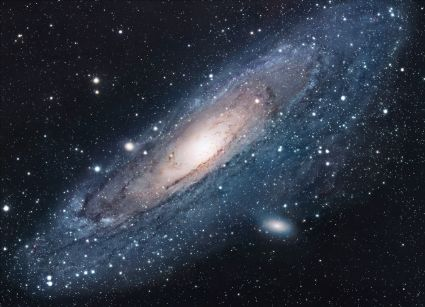
\includegraphics{universe}


\pagebreak


ok now here is a much more better placed beautiful picture of a mathematical penis:
\begin{figure}[htbp]
    \centering
    % 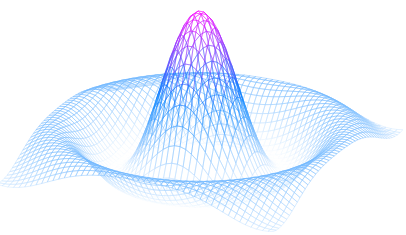
\includegraphics{mesh}
    \begin{equation}
        \frac{b+-\sqrt[2]{b^{2}-4(ac)}}{2ab}
    \end{equation}
    \caption{the quartratic formula}
    \label{eq:quadratic_formula}
\end{figure}

\begin{figure}[htbp]
    \centering
    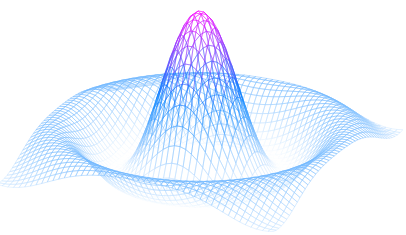
\includegraphics{mesh}
    \caption{A mathematical penis}
    \label{fig:peen}
\end{figure}

okay, so figure \ref{fig:peen} is the peen and its on page \pageref{fig:peen}, but figure \ref{eq:quadratic_formula} is the quadratic formula and is on page \pageref{eq:quadratic_formula}, check if its right!

\pagebreak

okay, up next is lists

\begin{itemize}
    \item this is an item
    \item and this is another item
        \item damn this is convenient (this is actually put on after an indent)
    \item oh it appears that it does not matter
        \item it will still just be aligned, I mean it should be; its the whole purpose
\end{itemize}



okay so apparently when you can do the \$ math here \$ in a whole new line!
like this:
but you can add numbers by just using the standard \\begin{equation} thingy like this:
\begin{equation}
    E=mc^{2}
    \label{eq:eins}
\end{equation}
Take that einstein!

wait what if we put the \\begin{} ones in line
    like \begin{equation} E=mc^{2} \label{eq:einst} \end{equation} so its like in one line?

    yeah okay it does not want to be in one line. also its not \\begin{equation}, its \\begin{MATH} for inline, which is completely unnecessary to write that much anyways
but let me guess the previous equation number is \ref{eq:einst} right? and the first one is \ref{eq:eins}. Did I get that right too??

yeah dumbass cuz I'm cheating with the \\label trick 


lets see if there is any difference if I try to use the \\(  \\) instead of the \$ \$
here is the famous \(a^{2} + b^{2} = c^{2}\)

lemme try some integrals
\begin{equation}
    \int_{freedom}^{stoiene}
    \pagebreak
    \int \frac{\texttt{d}x}{\texttt{d}t}=\texttt{sum stuff here idk lol}
\end{equation}

\end{document}

